% begin module polar-intersection-ex3
\begin{frame}
\begin{example} %[Example 3, p. 688]
Find all points of intersection of the polar curves $r = \frac{1}{2}$ and $r = \cos 2\theta$.
\begin{columns}[c]
\column{.4\textwidth}
\ \only<handout:0| -3>{%
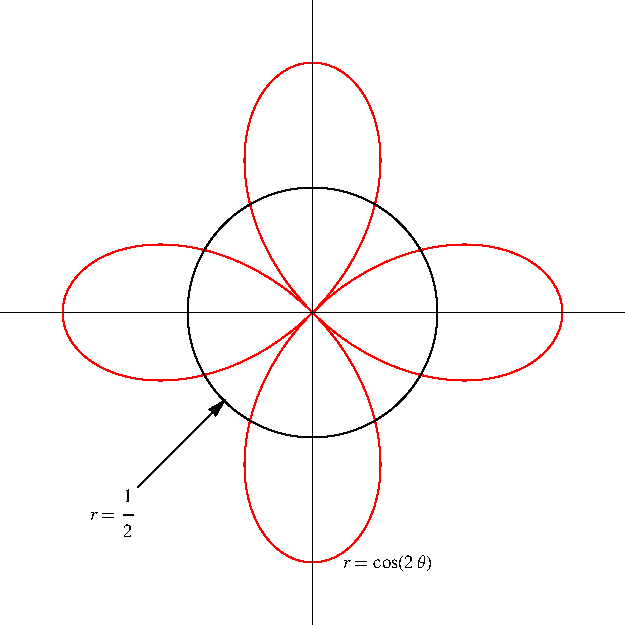
\includegraphics[height=5cm]{polar-curves/pictures/11-04-ex3a.pdf}%
}%
\only<handout:0| 4-5>{%
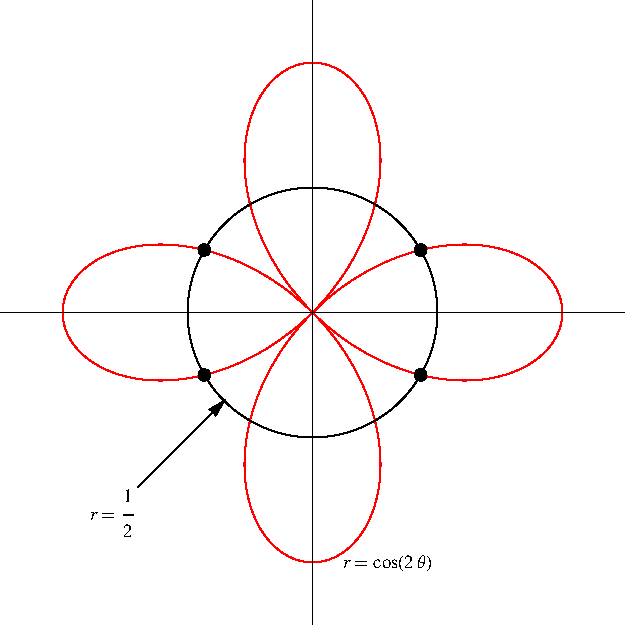
\includegraphics[height=5cm]{polar-curves/pictures/11-04-ex3b.pdf}%
}%
\only<6-8>{%
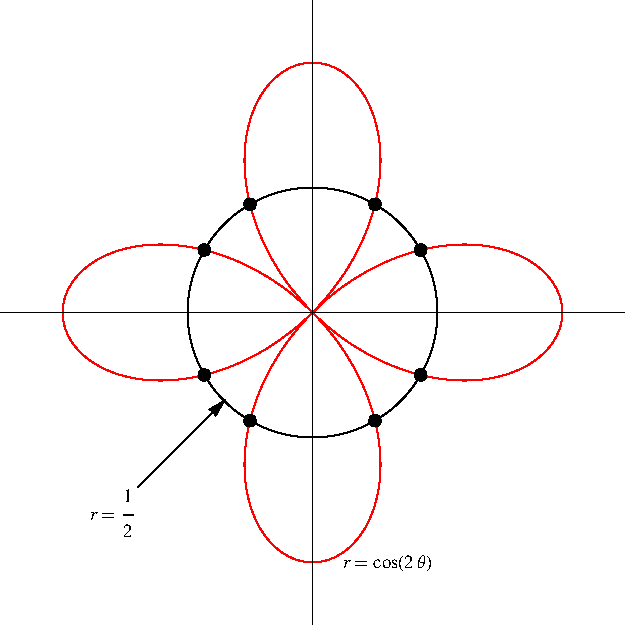
\includegraphics[height=5cm]{polar-curves/pictures/11-04-ex3c.pdf}%
}%
\only<handout:0| 9>{%
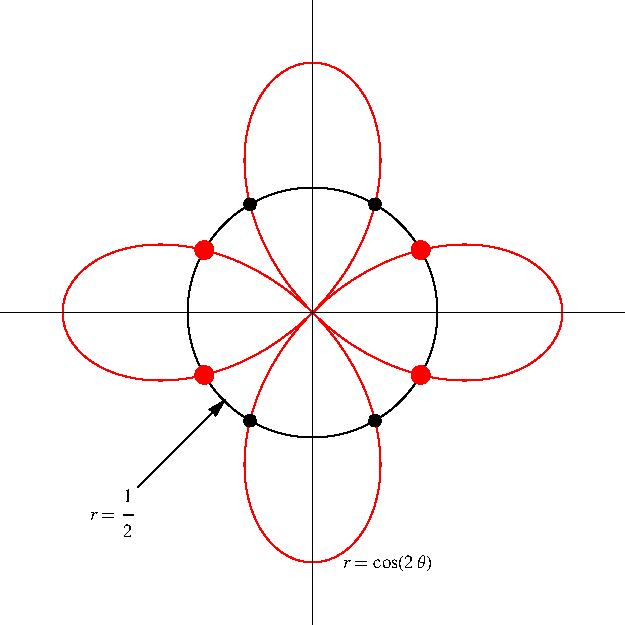
\includegraphics[height=5cm]{polar-curves/pictures/11-04-ex3d.pdf}%
}%
\only<handout:0| 10->{%
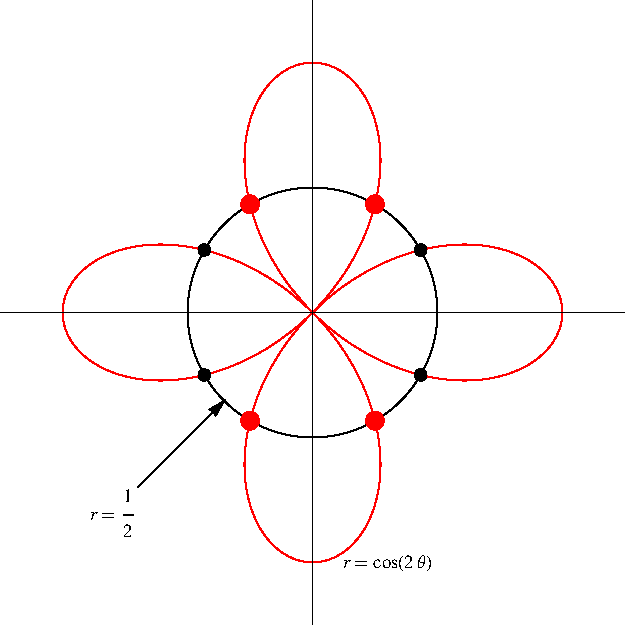
\includegraphics[height=5cm]{polar-curves/pictures/11-04-ex3e.pdf}%
}%

\column{.6\textwidth}
\abovedisplayskip=0pt
\belowdisplayskip=0pt
\begin{eqnarray*}
\uncover<2->{%
\cos 2\theta%
}%
& \uncover<2->{ = } &%
\uncover<2->{%
\frac{1}{2}%
}\\%
\uncover<3->{%
2\theta%
}%
& \uncover<3->{ = } &%
\uncover<3->{%
\frac{\pi}{3}, \frac{5\pi}{3}, \frac{7\pi}{3}, \frac{11\pi}{3}%
}\\%
\uncover<4->{%
\theta%
}%
& \uncover<4->{ = } &%
\uncover<4->{%
\frac{\pi}{6}, \frac{5\pi}{6}, \frac{7\pi}{6}, \frac{11\pi}{6}%
}%
\end{eqnarray*}
\begin{itemize}
\item<5->  This only gives four points.
\item<6->  There are actually eight.
\item<7->  The circle $r = \frac{1}{2}$ also has polar equation $r = -\frac{1}{2}$.
\item<8->  To find all eight points, solve \alert<handout:0| 9>{$\cos 2\theta = \frac{1}{2}$} and \alert<handout:0| 10>{$\cos 2\theta = -\frac{1}{2}$}.
\end{itemize}
\end{columns}
\end{example}
\end{frame}
% end module polar-intersection-ex3
